%%% -*- TeX-engine: xetex -*-
\documentclass{beamer}

% for themes, etc.
\usepackage{times}  % fonts are up to you
\usepackage{graphicx}
\usepackage{color}
\usepackage{hyperref}

\mode<presentation>
{
  \usetheme{Warsaw}
  \useoutertheme{infolines}
  \usecolortheme{whale}
  \setbeamertemplate{navigation symbols}{}
}
\usepackage{fontspec}
\usepackage{xunicode}
\usepackage[BoldFont,SlantFont]{xeCJK}
\setCJKmainfont{SimSun}
\setCJKmonofont{SimHei}

\title{
  基于翻译技术的流量调度研究 \\
  结题报告
}
\author{王文鑫}
\date{2016年6月8日}

\AtBeginSection[]
{
  \begin{frame}<beamer> 
    \tableofcontents[currentsection]
  \end{frame}
}
\setbeamertemplate{caption}{\raggedright\insertcaption\par}

\begin{document}

\begin{frame}
  \titlepage
\end{frame}

\section{研究课题}

\begin{frame}
  \frametitle{研究课题}

  \vspace{-1em}
  \begin{figure}
    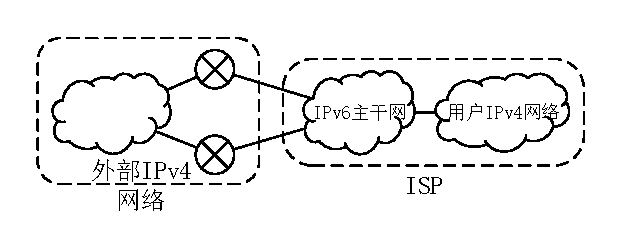
\includegraphics[width=0.9\textwidth]{figs/0-purpose.pdf}
  \end{figure}
  \vspace{-2em}

  \begin{block}{主要工作内容}
    \begin{itemize}
    \item 在IPv4/IPv6过渡场景中,基于翻译等过渡技术,设计和实现灵活通用的流量调度机制
    \item 使得ISP可以自由定制多出口情景下的调度策略
      \begin{itemize}
      \item 负载均衡、容错
      \end{itemize}
    \end{itemize}
  \end{block}
\end{frame}

\section{研究背景和研究思路}
\subsection{IPv4/IPv6过渡}
\begin{frame}
  \frametitle{过渡技术}
  \vspace{-1em}
  \begin{figure}
    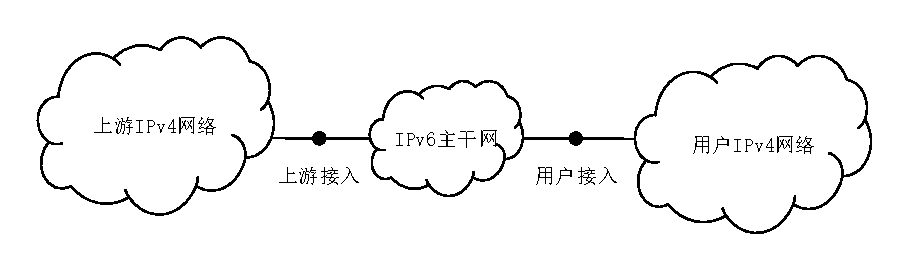
\includegraphics[width=\textwidth]{figs/1-464.pdf}
  \end{figure}
  \vspace{-2em}

  \begin{block}{从IPv4到IPv6}
    \begin{itemize}
    \item IPv4地址池已于2011年2月3日枯竭\footnotemark[1]
    \item IPv4到IPv6的切换是一个渐进的过程
    \item 保证升级过程中对原始IPv4应用的支持,促进IPv6网络的扩展
    \item 课题研究的过渡场景:使用IPv6主干网承载IPv4端到端通信
    \end{itemize}
  \end{block}

  \footnotetext[1]{https://www.nro.net/news/ipv4-free-pool-depleted}
\end{frame}

\begin{frame}
  \frametitle{DIVI、NAT64、DS-Lite}

  \vspace{-1.5em}
  \begin{figure}
    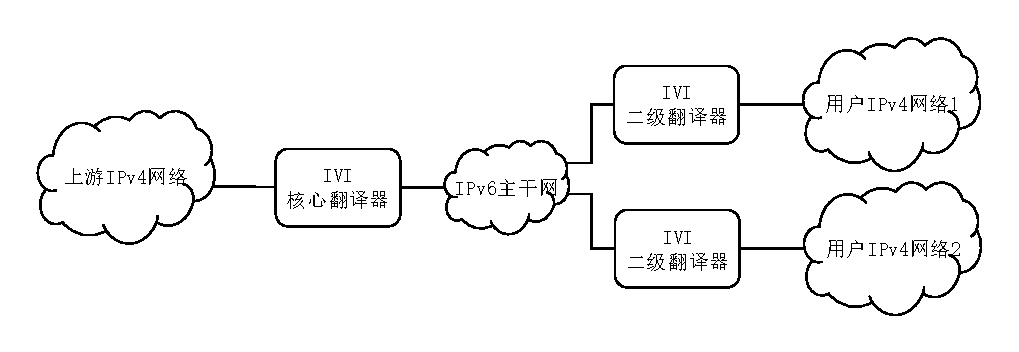
\includegraphics[width=0.93\textwidth]{figs/5-divi.pdf}\\
    \vspace{-3.5em}
    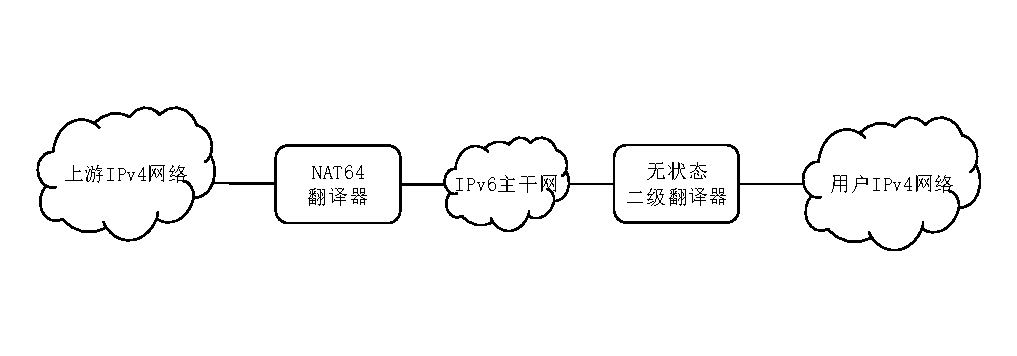
\includegraphics[width=0.93\textwidth]{figs/7-nat64.pdf}\\
    \vspace{-4em}
    \caption{\tiny DIVI无状态翻译和NAT64有状态翻译}
    \vspace{-2em}
    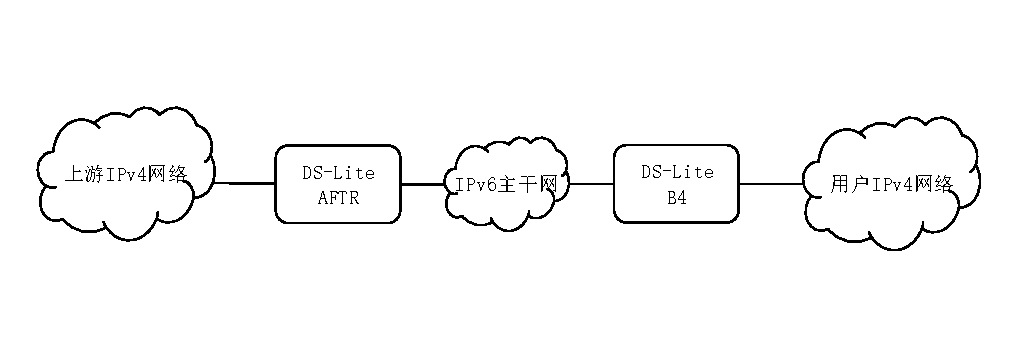
\includegraphics[width=0.93\textwidth]{figs/8-ds-lite.pdf}
    \vspace{-4em}
    \caption{\tiny DS-Lite封装}
  \end{figure}
\end{frame}

\subsection{多出口流量调度}
\begin{frame}
  \frametitle{多出口流量调度}

  \begin{block}{多出口的作用}
    \begin{itemize}
    \item 优化带宽利用率、成本,主备切换……
    \item 搭建不同过渡系统,优势互补
    \item 按照一定的策略引导用户流量进入不同的上游网络
    \end{itemize}
  \end{block}

  \begin{block}{调度机制}
    \begin{itemize}
    \item 传统IPv4网络:BGP、策略路由
    \item 过渡场景:用户的IPv4流量先在用户接入口汇聚
    \item 将流量导向不同的过渡系统,从而选择上游出口
    \end{itemize}
  \end{block}
\end{frame}

\begin{frame}
  \begin{figure}
    \vspace{-1em}
    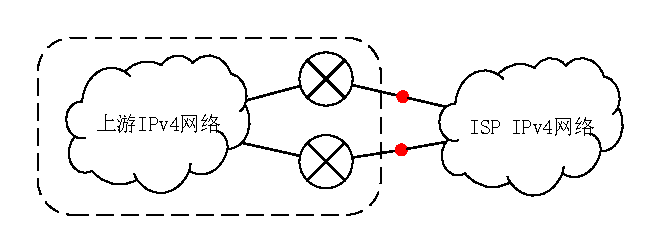
\includegraphics[width=0.8\textwidth]{figs/20-ipv4-multi-egress.pdf}
    \vspace{-2em}
    \caption{\tiny 传统IPv4网络中的流量调度}
    \vspace{-1em}
    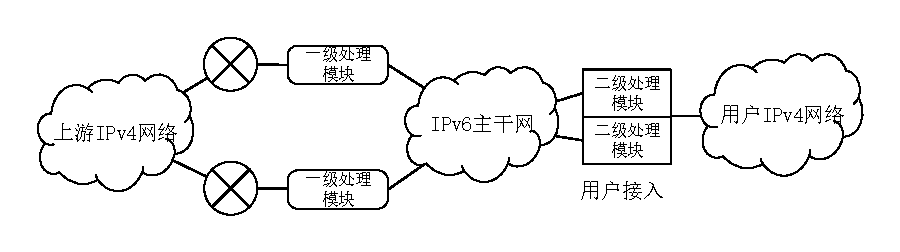
\includegraphics[width=\textwidth]{figs/21-ipv6-multi-egress.pdf}
    \vspace{-2em}
    \caption{\tiny 过渡场景下的流量调度}
  \end{figure}
\end{frame}

\subsection{总体思路}
\begin{frame}
  \frametitle{总体思路}

  \begin{block}{方案}
    \begin{itemize}
    \item 在用户接入口处设计和实现调度机制
      \begin{itemize}
      \item 灵活:基于五元组
      \item 通用:与具体过渡技术解耦
      \end{itemize}
    \item 修改现有过渡技术,适配多出口场景
    \item 测试和验证
    \end{itemize}
  \end{block}
\end{frame}

\section{设计和实现}
\subsection{总体结构}
\begin{frame}
  \frametitle{总体结构}
  \vspace{-1em}

  \begin{figure}
    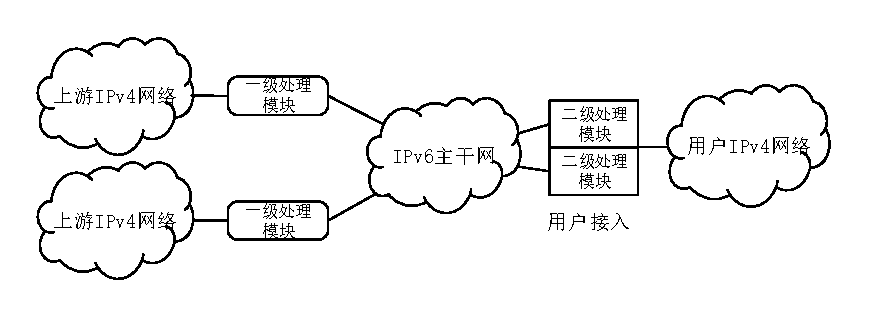
\includegraphics[width=\textwidth]{figs/9-multi-egress.pdf}
  \end{figure}
  \vspace{-1em}

  \begin{block}{设计思路}
    \begin{itemize}
    \item 用户接入口负责分发流量到二级处理模块,从而对应一级模块进入不同上游接入
    \item 正确:各模块共存时能够正常工作
    \item 高效:用户流量在千兆或者万兆级别,间接代价被流量放大
    \item 通用:与具体过渡技术解耦,不依赖内部实现
    \end{itemize}
  \end{block}
\end{frame}

\subsection{各模块设计}
\begin{frame}
  \frametitle{用户网接入点结构设计}
  \begin{figure}
    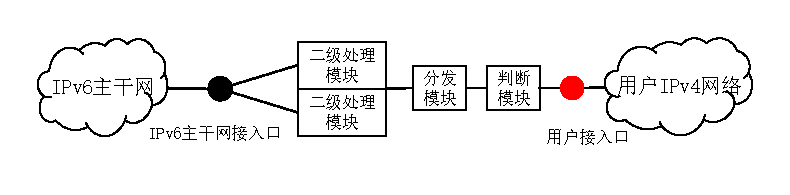
\includegraphics[width=\textwidth]{figs/10-user-access-point-a.pdf}
  \end{figure}
  \vspace{-1em}

  \begin{block}{用户IPv4接入网口}
    \begin{itemize}
    \item DHCP服务:分发用户IPv4地址
    \item DNS服务:域名解析
      \begin{itemize}
      \item 不涉及地址翻译,多级查询依赖过渡技术
      \end{itemize}
    \end{itemize}
  \end{block}

  \begin{block}{用户IPv6接入网口}
    \begin{itemize}
    \item 不受限制:RA、DHCPv6、DNS
    \end{itemize}
  \end{block}
\end{frame}

\begin{frame}
  \frametitle{用户网接入点结构设计}
  \begin{figure}
    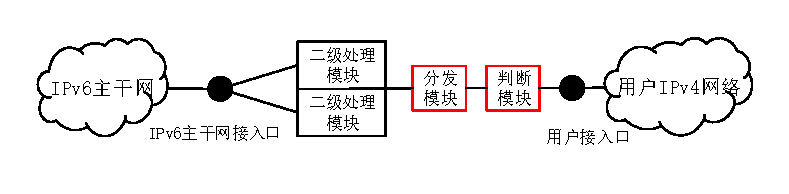
\includegraphics[width=\textwidth]{figs/10-user-access-point-b.pdf}
  \end{figure}
  \vspace{-1em}

  \begin{block}{判断模块}
    \begin{itemize}
    \item 根据五元组信息,判断数据包发往某个二级处理模块
    \item 通过标记数据包实现(见后)
    \end{itemize}
  \end{block}

  \begin{block}{分发模块}
    \begin{itemize}
    \item 根据决策,将数据包发往不同的二级处理模块
    \end{itemize}
  \end{block}
\end{frame}

\begin{frame}
  \frametitle{用户网接入点结构设计}
  \begin{figure}
    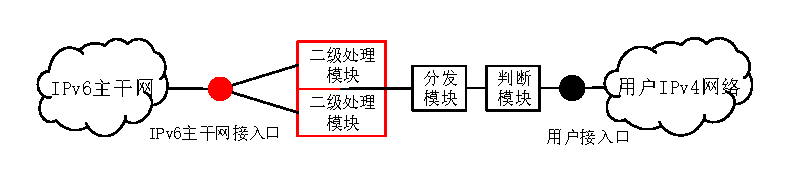
\includegraphics[width=\textwidth]{figs/10-user-access-point-c.pdf}
  \end{figure}
  \vspace{-1em}

  \begin{block}{各二级处理模块}
    \begin{itemize}
    \item 需要为调度机制提供可控的数据包传入口
    \item 二级模块间路由等规则的冲突解决
    \end{itemize}
  \end{block}

  \begin{block}{IPv6主干网接入网口}
    \begin{itemize}
    \item 所有二级模块共享一个主干网接入网口
    \end{itemize}
  \end{block}
\end{frame}

\subsection{各模块实现}
\begin{frame}
  \frametitle{用户网接入系统实现}
  \vspace{-1em}
  \begin{figure}
    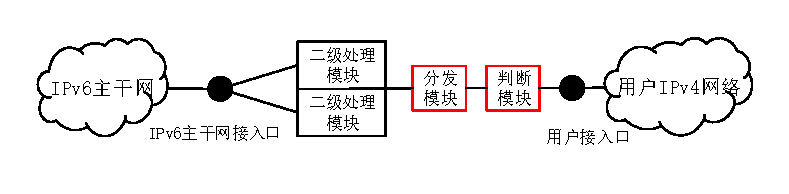
\includegraphics[width=0.7\textwidth]{figs/10-user-access-point-b.pdf}
  \end{figure}
  \vspace{-3em}
  \begin{figure}
    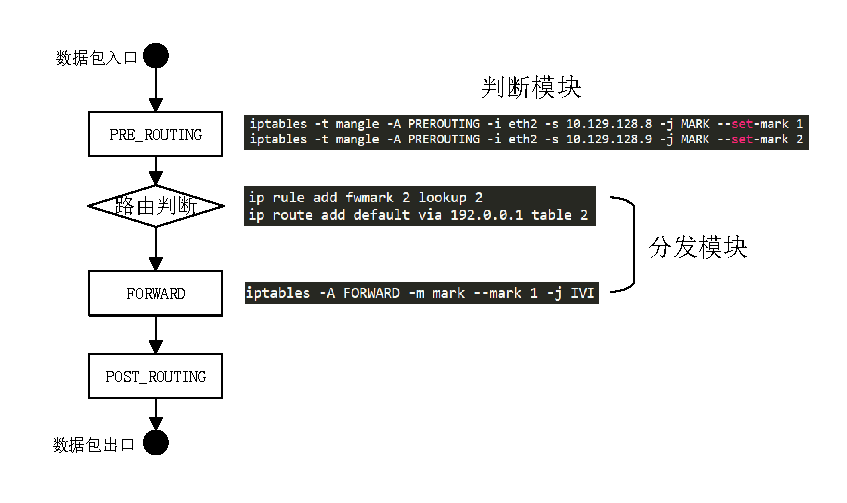
\includegraphics[width=\textwidth]{figs/11-netfilter.pdf}
  \end{figure}
  \vspace{-2em}

\end{frame}

\begin{frame}
  \frametitle{用户网接入系统实现}
  \vspace{-1em}
  \begin{figure}
    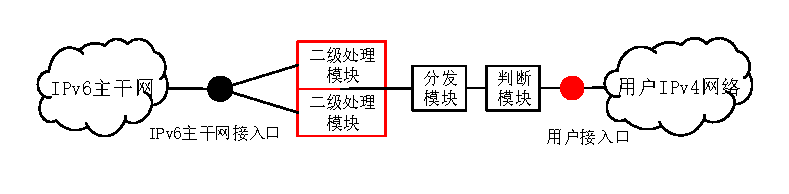
\includegraphics[width=\textwidth]{figs/10-user-access-point-d.pdf}
  \end{figure}
  \vspace{-2em}

  \begin{block}{各二级处理模块}
    \begin{itemize}
    \item 提供服从调度需求的数据接口
      \begin{itemize}
      \item 扩展DIVI二级处理器:从Netfilter实现迁移至IPTables
      \item 添加NAT64无状态二级处理器:IPTables
      \end{itemize}
    \end{itemize}
  \end{block}

  \begin{block}{无法避免的冲突}
    \begin{itemize}
    \item 将有冲突的模块隔离在Linux命名空间
    \item 各空间仿佛是独立的计算机,使用虚拟以太网线链接
    \item 在全局空间外,使用路由规则调度即可
    \end{itemize}
  \end{block}
\end{frame}

\section{测试和验证}

\begin{frame}
  \frametitle{测试平台}
  \vspace{-1em}
  \begin{figure}
    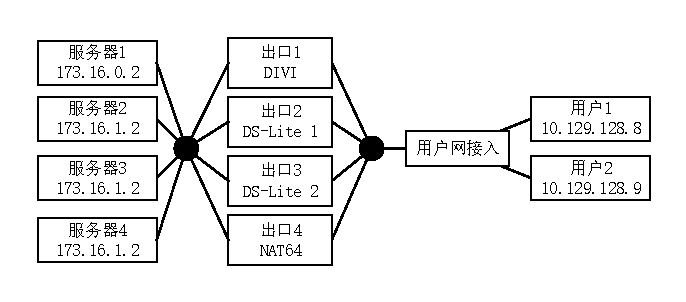
\includegraphics[width=\textwidth]{figs/12-test-arch.pdf}
  \end{figure}
  \vspace{-2em}

  \begin{table}
    \begin{tabular}{l | l}
      一级处理器 & 上游IPv4地址(段)\\
      \hline
      IVI核心翻译器 & 58.200.129.128/27\\
      DS-Lite AFTR1 & 198.18.200.1\\
      DS-Lite AFTR2 & 198.18.201.1\\
      NAT64一级翻译器 & 198.18.202.1\\
    \end{tabular}
  \end{table}
\end{frame}

\begin{frame}
  \frametitle{基于源和目标地址的流量调度}
  \vspace{-1em}
  \begin{figure}
    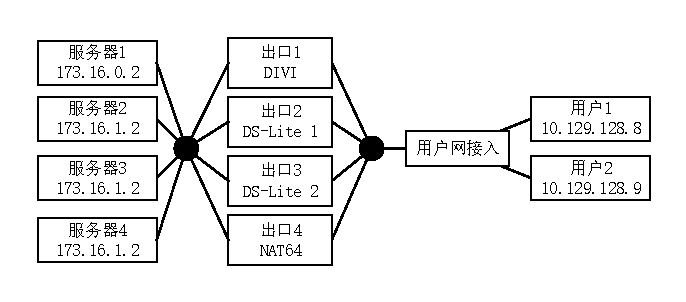
\includegraphics[width=\textwidth]{figs/12-test-arch.pdf}
  \end{figure}
  \vspace{-2em}

  \begin{block}{策略}
    \begin{itemize}
    \item 用户1所有流量均通过上游出口1(DIVI)(基于源地址的调度)
    \item 用户2与服务器1/2/3/4的通信分别通过上游出口1/2/3/4(基于目标地址的调度)
    \end{itemize}
  \end{block}
\end{frame}

\begin{frame}
  \frametitle{节选测试结果}

  \begin{figure}
    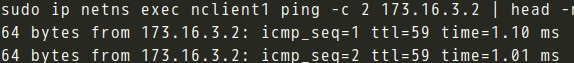
\includegraphics[width=0.7\textwidth]{figs/c1-s4-ping.jpeg}\\
    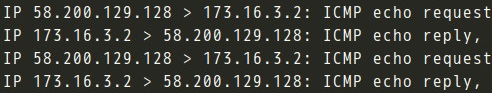
\includegraphics[width=0.7\textwidth]{figs/c1-s4-pdump.jpeg}
    \caption{\tiny 基于源地址的调度}
  \end{figure}

  \vspace{-1em}

  \begin{figure}
    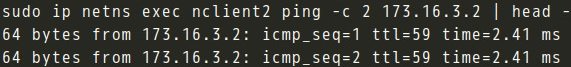
\includegraphics[width=0.7\textwidth]{figs/c2-s4-ping.jpeg}\\
    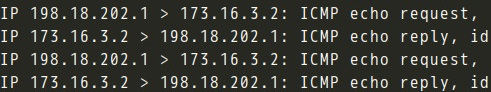
\includegraphics[width=0.7\textwidth]{figs/c2-s4-pdump.jpeg}
    \caption{\tiny 基于目的地址的调度}
  \end{figure}
\end{frame}

\section{总结}
\begin{frame}
  \frametitle{总结和计划}

  \begin{block}{主要贡献}
    \begin{itemize}
    \item 设计调度机制,使得过渡场景下的流量调度成为可能
      \begin{itemize}
      \item 与具体过渡技术解耦的(通用),基于五元组(灵活)
      \item ISP通过制定调度策略,优化用户体验,降低管理成本
      \end{itemize}
    \item 扩展过渡技术,符合多出口场景的需求
    \end{itemize}
  \end{block}

  \begin{block}{后续工作}
    \begin{itemize}
    \item 在实际场景中测试,获取性能指标
    \item 利用调度机制研发流量调度应用解决实际需求
    \end{itemize}
  \end{block}
\end{frame}

\section{参考文献}
\begin{frame}
  \frametitle{参考文献}
  \begin{itemize}
  \item \href{https://tools.ietf.org/html/rfc7599}{RFC7599}
  \item \href{https://tools.ietf.org/html/rfc7597}{RFC7597}
  \item \href{https://tools.ietf.org/html/rfc6219}{RFC6219}
  \item \href{https://tools.ietf.org/html/rfc6052}{RFC6052}
  \item \href{https://tools.ietf.org/html/rfc7598}{RFC7598}
  \item \href{http://www.netfilter.org}{The netfilter.org project}
  \end{itemize}
\end{frame}

\section{Q\&A}

\begin{frame}
  \frametitle{Q\&A}
  \begin{center}
    {\LARGE 谢谢!}
    \vspace{3em}
    {\LARGE 请老师们提问和指导!}
  \end{center}
\end{frame}
\end{document}